\chapter{ExpressJS}

Express edo ExpressJS \index{express} kode irekiko Node-rako web aplikazio dinamikoak programatzeko \textit{framework} bat da. Kapitulu honetan adibide batekin egingo dugu lan: bezeroen datuak kudeatzeko aplikazio sinple bat programatuko dugu, hasiera-hasieratik.

Bezeroen izen-abizenak eta helbidea elektronikoa gorde, editatu, ezabatu eta bistaratzeko inprimaki bat izango dugu. Lehendabiziko bertsioan datu horiek soilik memorian gordeko ditugu. Bigarren bertsioan, bezeroen datuak \textit{noSQL}\index{noSQL} motako datu-base batean gordeko ditugu (\textit{mongodb}\index{mongodb} izeneko datu-base batean, hain zuzen ere).

Has gaitezen, lehenengo eta behin, \textit{express} \textit{framework}-a instalatzen.

Lehenengo eta behin aplikazioa hasieratu beharko dugu, \hl{npm init} komandoaz.


\begin{lstlisting}[language=Bash,numbers=none]
$ npm init
Aplikazioaren izena: bezeroak
Bertsioa: 1.0
Deskribapena: bezeroen kudeaketa
Entry Point (nondik hasten den aplikazioa): app.js
Testak egiteko komandoa: momentuz hutsik
Git reepo: momentuz hutsik
keywords: hitz gakoak, momentuz hutsik
author: zure izena
lizentzia: momentuz hutsik

\end{lstlisting}

\textit{npm init} komandoa exekutatu ondoren, \textit{package.json} fitxategia sortuko da.

Jarraian, \textit{express} eta haren mendekotasun guztiak instalatuko ditugu:

\begin{lstlisting}[language=Bash,numbers=none]
$ npm install express --save
\end{lstlisting}

Bukatzeko, HTTP zerbitzari sinple bat programatuko dugu:

\begin{lstlisting}[language=JavaScript]
// app.js fitxategia

let express = require('express');
let path = require('path');

let app = express();
app.listen( 3000, function() {
	console.log("Zerbitzaria 3000 portuan entzuten");
})
\end{lstlisting}

Zerbitzaria martxan jartzeko, \hl{node app.js} komandoa landuko dugu.

Orain http://localhost:3000/ URLan sartzen bagara, erantzun bat jasoko dugu, baina ziur asko ez da guk espero dugun erantzuna izango:

\begin{lstlisting}[numbers=none]
"Cannot GET /"
\end{lstlisting}

Erroreak esan nahi du zerbitzariak ez dakiela nola erantzun bidali diogun GET\index{GET} motako eskaerari. Alegia, \textit{"/"} bidea (\textit{route})\index{route} ez dugula tratatu zerbitzarian.  GET motako bideak tratatzeko, metodo berri bat programatu behar dugu:

\begin{lstlisting}[language=JavaScript]
app.get("/", function(req, res) {
	res.send("Kaixo mundua!");
});
\end{lstlisting}

Orain bai, URL bera eskatzean (http://localhost:3000/), ``Kaixo mundua!'' mezua jasoko dugu erantzun gisa.

\begin{alertinfo}{Zer da \texttt{-{}-}save aukera?}
  \index{--save}\texttt{-{}-}save aukerarekin instalatu nahi dugun paketea package.json fitxategian mendekotasun gisa idatzi nahi dugula zehazten dugu. \texttt{-{}-}save aukera erabili ezean, mendekotasun-paketea gure ordenagailuan instalatuko da, baina ez dugu horren berri izango package.json fitxategian (alegia, beste garatzaileek ez dute jakingo mendekotasun hau gure aplikaziorako beharrezkoa dela).
\end{alertinfo}

\section{Baliabide estatikoak}

\index{app.get()}\textit{app.get()} edo \index{app.post()} \textit{app.post()} erabili behar dugu edozein HTML orria zerbitzatzeko? Ezin dugu HTML5en egindako orri estatiko bat zerbitzatu beste modu egokiago batean? Noski, horretarako \textit{express} aplikazioaren bideraketak zehaztu baino lehen (app.get, app.post zehaztu baino lehen) baliabide estatikoen karpeta non dagoen adierazi beharko dugu (kasu honetan, \textit{public} izeneko karpeta):

\begin{lstlisting}
app.use(express.static('public'))
\end{lstlisting}

\index{app.use}\textit{app.use} egiturari \index{middleware}\textit{middleware} deitzen zaio. Bideraketak baino lehenago egin behar diren beste ataza eta prozesuak zehaztuko ditugu middleware funtzioekin. Hurrengo ataletan gehiago sakonduko dugu middleware honetan, baina momentuz horrela utziko dugu.

Adibide gisa, \textit{public} karpetan orri estatiko hau utziko dugu, inprimaki sinple batekin, \textit{post.html} izenarekin:

\begin{lstlisting}

<!DOCTYPE html>
<html lang="en">
<head>
	<meta charset="UTF-8">
	<title>POST metodoa erabiltzen duen inprimakia</title>
</head>
<body>
<form action="/bezeroa" method="POST">
Izena: <input type="text" name="izena"><input type="submit" value="Bidali">
</form>
</body>
</html>
\end{lstlisting}

Nabigatzailean orri hori atzitzeko hurrengo URLa idatziko dugu:

\hl{http://localhost:3000/post.html}

Ohart zaitez URLan ez dugula \hl{public/post.html} idatzi. \textit{Express}-ek badaki besterik ezean, HTML orriaren fitxategi estatikoak public/ karpetan egon behar duela.

\section{GET parametroak URLan bidaltzen}

Nola bidali ahal diogu gure \textit{express} aplikazioari GET parametro bat? Alegia, demagun horrelako URL bat idatzita: http://localhost:3000/bezeroa/Oihane zerbitzariak eskaera jaso eta ``Kaixo Oihane'' mezuarekin erantzun behar duela (ikus \ref{fig:urlparametroak}. irudia). URLan agertzen den izena jasotzeko \textit{req.params}\index{req.params} objektua erabiliko dugu, honela:

\begin{lstlisting}
app.get('/bezeroa/:izena', function(req, res) {
  res.send("Bezeroaren izena: " + req.params.izena);
});
\end{lstlisting}

\begin{figure}[ht]
	\centering
\begin{tikzpicture}[framed]
\node[anchor=south west,inner sep=0] (image) at (0,0)
   {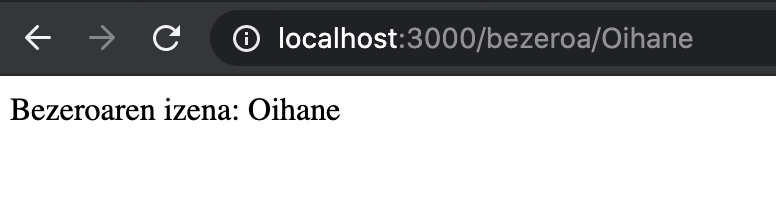
\includegraphics[trim=0cm 0cm 0cm 0cm, clip=true, width=0.75\textwidth]{img/urlparametroak.png}};
\end{tikzpicture}
\caption{URL batean bidaltzen diren parametroak (\textit{URL parameters}) jaso eta tratatu ahal dira \textit{req.params} erabiliz.}
\label{fig:urlparametroak}
\end{figure}


\section{GET parametroak eskaeran bidaltzen}
GET metodoan parametroak URLan bi modutara bidal daitezke: URL bidearen parte izanik (ikusi dugun bezala) edo URLaren azken zatian, eskaera (\textit{query string}\index{query string}) izeneko parametroetan, galdera-ikur baten ostean, honela:\newline
\href{http://localhost:3000/bezeroa/?izena=Oihane}{http://localhost:3000/bezeroa/?izena=Oihane}.

Eskaera-parametro horiek jasotzeko, \textit{req.params}\index{req.params} erabili ordez, \textit{req.query}\index{req.query} erabiliko dugu. Adibidez:

\begin{lstlisting}
app.get('/bezeroa', function(req, res) {
  res.send("Bezeroaren izena: " + req.query.izena);
});
\end{lstlisting}

Parametro bat baino gehiago bidali nahi izanez gero, aldagaiak \hl{\&} karaktereaz banatuko ditugu, honela: \href{http://localhost:3000/bezeroa/?izena=Oihane\&abizena=Pereira}{http://localhost:3000/bezeroa/?izena=Oihane\&abizena=Pereira}.

\begin{lstlisting}
app.get('/bezeroa', function(req, res) {
  res.send("Bezeroaren izena: " + req.query.izena);
  res.send("Bezeroaren abizena: " + req.query.abizena);
});
\end{lstlisting}

\section{POST parametroak}\index{POST}

Inprimaki baten datuak orokorrean POST bidez bidaltzen dira, ez GET bidez. Nola jaso POST balio horiek zerbitzarian? Eskaera (\textit{request}) baten \textit{body} atributuan daude parametro hauek. Adibidez, \index{req.body}\textit{req.body.izena}. Baina, besterik gabe, hau inplementatzen badugu:

\begin{lstlisting}
app.post('/bezeroa', function(req, res) {
    res.send("Bezeroaren izena:" + req.body.izena;
}
\end{lstlisting}

ez dugu ezer jasoko. Zergatik? Arazoa da POST parametroak bide edo \textit{route} batean sartu baino lehen tratatu egin behar direla. Nabigatzaileak bidaltzen dituen datuak zerbitzarian jaso eta bideratu baino lehen tratatu egin nahi baditugu, \textit{express}-en middleware izeneko funtzioak erabili beharko ditugu.

Middleware bat erabiltzeko, aurreko gaian ikusi dugunez, \textit{app.use(funtzioa)} erabiliko dugu, bideraketak egin baino lehen. Kasu honetan, \index{body.parser}\textit{body.parser} izeneko middlewarea erabili genezake POST bidez datozen parametroak tratatzeko. Hala ere, ez da beharrezkoa izango, Express 4.16 bertsiotik aurrera, \index{body.parser}\textit{body.parser} middleware hau jada integratuta dago.
Beraz, nahikoa da ondorengoa egitea:

\begin{lstlisting}[language=JavaScript]
// application/x-www-form-urlencoded
app.use(express.urlencoded({ extended: true }))
\end{lstlisting}

Horrekin aurreko kodeak ondo funtzionatuko du. 

\begin{lstlisting}[language=JavaScript]
// parseatu  application/x-www-form-urlencoded datuak
app.use(express.urlencoded({ extended: true }))
app.post('/bezeroa', function(req, res) {
    res.send("Bezeroaren izena:" + req.body.izena;
}
\end{lstlisting}

\begin{alertinfo}{x-www-form-urlencoded}
\ref{fig:form-urlencoded}. irudian ikusten dugunez, form baten datuak POST bidez bidaltzean, besterik ezean, HTTP eskaeraren eduki mota (Content-Type) application/x-www-form-urlencoded izango da.
\end{alertinfo}





% \begin{figure}[ht]
% 	\centering
% \begin{minipage}{.4\textwidth}
% \begin{tikzpicture}[scale=0.5]
% \node[anchor=south west,inner sep=0] (image) at (0,0)
%    {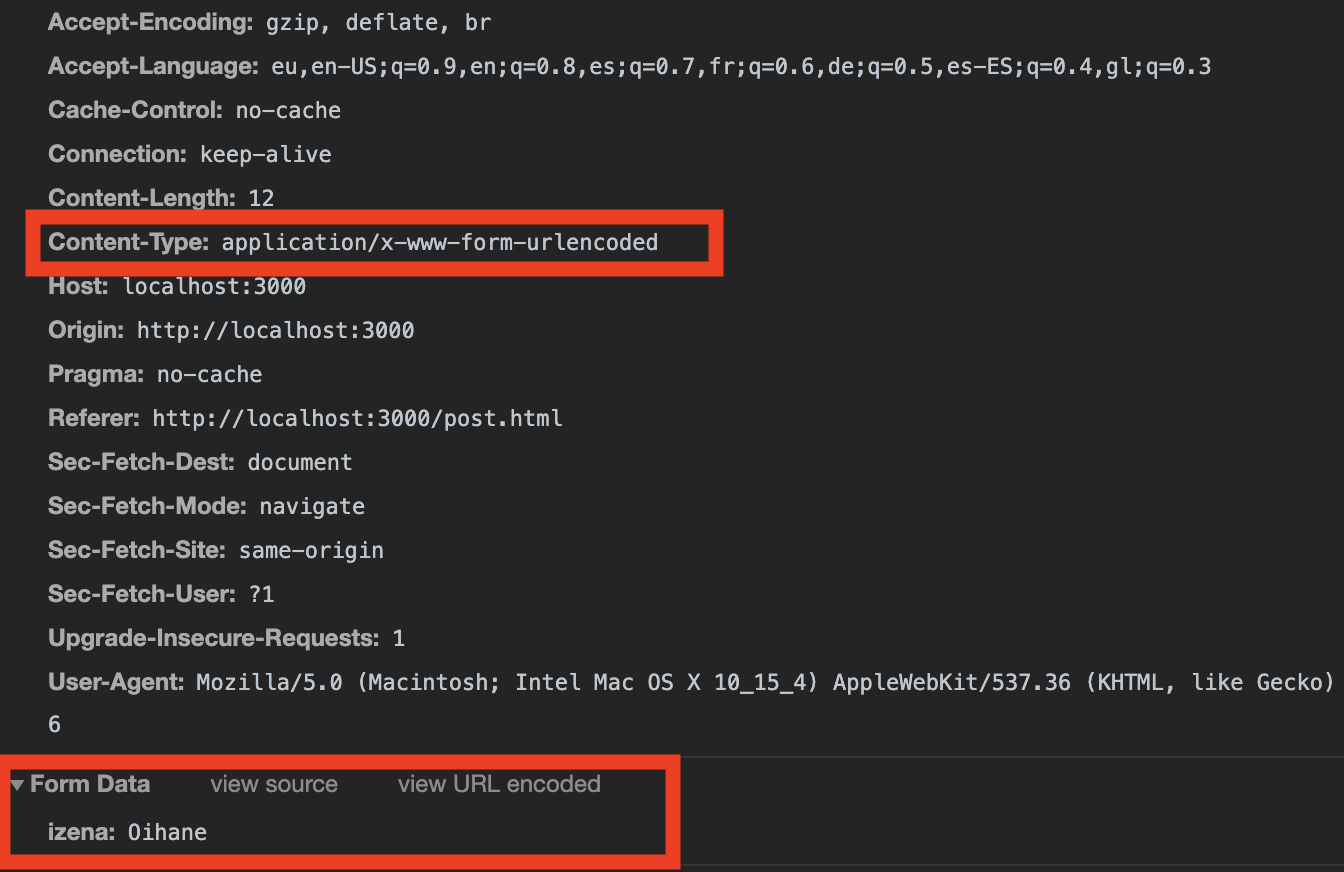
\includegraphics[trim=0cm 0cm 0cm 0cm, clip=true, width=1.0\textwidth]{img/form-urlencoded.png}};
% \end{tikzpicture} % pic 1
% \end{minipage}
% \begin{minipage}{.4\textwidth}
% \begin{tikzpicture}[scale=0.5]
% \node[anchor=south west,inner sep=0] (image) at (0,0)
%    {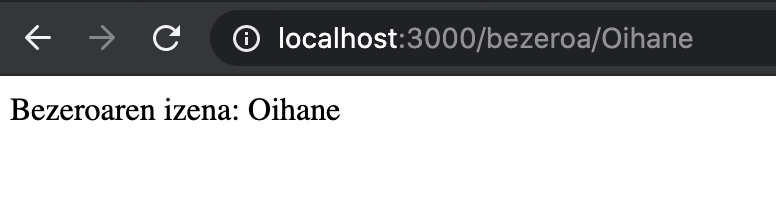
\includegraphics[trim=0cm 0cm 0cm 0cm, clip=true, width=1.0\textwidth]{img/urlparametroak.png}};
% \end{tikzpicture} % pic 2
% \end{minipage}
% \caption{xxxx}
% \label{fig:form-urlencoded}
% \end{figure}

\begin{figure}[ht]
	\centering
\begin{tikzpicture}[framed]
\node[anchor=south west,inner sep=0] (image) at (0,0)
   {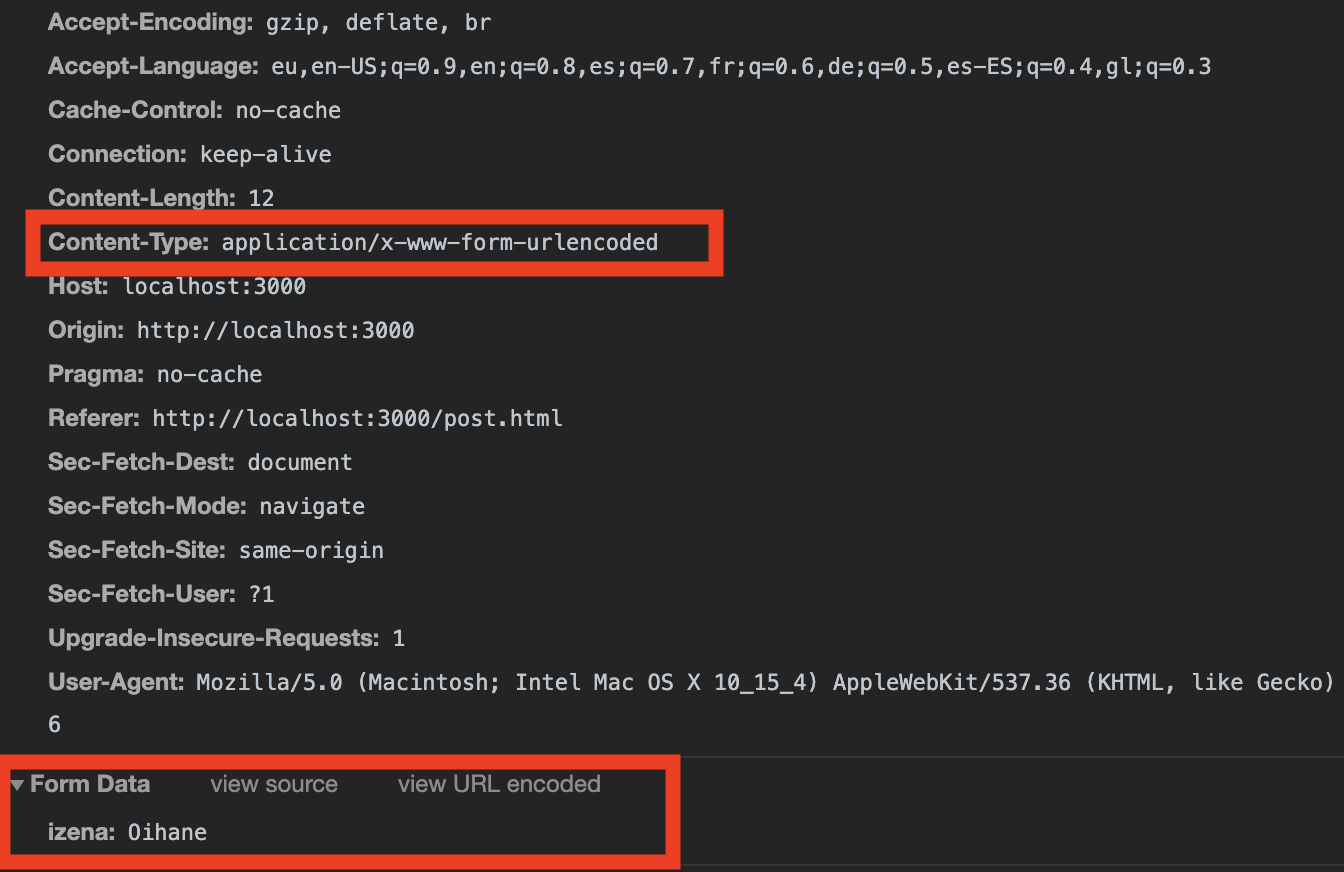
\includegraphics[trim=0cm 0cm 0cm 0cm, clip=true, width=0.75\textwidth]{img/form-urlencoded.png}};
\end{tikzpicture}
\caption{Form baten datuak bidaltzeko bi metodo daude: POST eta GET. GET kasuan, datuak URLan ikusiko dira. POST kasuan, HTTP eskaeraren edukian joango dira eta eskaeraren eduki mota \textit{application/x-www-form-urlencoded} izango da.}
\label{fig:form-urlencoded}
\end{figure}

\section{Nodemon}\index{nodemon}
Orain arte \hl{index.js} edo beste edozein JS fitxategitan aldaketa bat egitean, \textit{express} zerbitzaria itzali eta berriro martxan jarri behar izan dugu, aldaketak har zitzan. Baina edizio-prozesu hori oso astuna bilaka daiteke. Hoberena izango litzateke modulu bat izatea JS fitxategietan aldaketak automatikoki antzematen dituena eta berak bakarrik zerbitzaria berrabiarazten duena. Hori da, hain zuzen ere, \hl{nodemon} izeneko tresnaren zeregina. nodemon instalatzeko npm erabiliko dugu:

\begin{lstlisting}
$ npm install -g nodemon    
\end{lstlisting}

-g parametroak instalazio globala egin nahi dugula adierazten du. Hortik aurrera, erabiltzaile guztiek eskuragarri izango dute nodemon aplikazioa, ez soilik uneko erabiltzaileak. Behin instalatuta erabili egingo dugu:

\begin{lstlisting}
$ nodemon index.js
\end{lstlisting}

Orain, edozein aldaketa egiten badugu \hl{index.js} fitxategian, \textit{nodemon}-ek automatikoki aldaketa antzeman eta zerbitzaria automatikoki berrabiaraziko du. 

\section{Txantiloiak: EJS}\index{ejs}
Web garapenean diharduten enpresetan web programatzaileak eta web diseinatzaileak izaten dituzte. Orokorrean, programatzaileek aplikazioaren kodea programatzen dute eta diseinatzaileek web orrien itxura moldatzen dute, alegia, orrien diseinu grafikoa. Diseinatzaileek orri baten txantiloia prestatzen dute gero programatzaileek aplikazioaren datuekin betetzeko (adibidez, datu-base batetik ekarritako datuekin). Express-ek ere HTML txantiloi baten gainean datuak bistaratzeko aukera ematen du. Izan ere, hainbat modulu daude txantiloiekin lan egiteko (\textit{ejs, pug, mustache, handlebars, jade}...). Liburu honetan ejs erabiliko dugu, erraza baita berarekin lan egitea.

Lehenengo eta behin, \textit{ejs} instalatu egin behar da:

\begin{lstlisting}
$ npm install ejs  --save
\end{lstlisting}

Jarraian, txantiloiak kudeatzeko ejs erabiliko dugula zehaztuko dugu (9. lerroan):

\begin{lstlisting}[language=JavaScript]
const express = require('express');
const path = require('path');
const bodyParser = require('body-parser')

const app = express();

app.use(express.static('public'))

app.set('view engine', 'ejs');
app.set('views', path.join(__dirname, 'views'));
\end{lstlisting}

10. lerroan txantiloiak zer karpetatan gordeko ditugun adierazten da (lerro horrek \textit{path} moduluarekin mendekotasun bat dauka, horregatik inportatu behar dugu 2. lerroan)

Orain, erro-katalogoa eskatzean, ez dugu zuzenean ``Kaixo mundua!'' katearekin erantzungo:

\begin{lstlisting}[language=JavaScript]
app.get("/", function(req, res) {
    res.send("Kaixo mundua!");
});
\end{lstlisting}

baizik eta, horren ordez, \hl{index.ejs} txantiloia bidaliko dugu:

\begin{lstlisting}
app.get("/", function(req, res) {
    res.render('index');
});
\end{lstlisting}

\hl{index.ejs} txantiloiaren edukian \ref{fig:ejs}. irudian daukagun kodea sartuko dugu, hots:

\begin{lstlisting}
<!doctype html>
<html lang="en">
<head>
    <meta charset="UTF-8">
    <title>EJS probatzen</title>
</head>
<body>
    Kaixo EJS txantiloi kudeatzailetik
</body>
</html>
\end{lstlisting}

\begin{figure}[ht]
	\centering
\begin{tikzpicture}[framed]
\node[anchor=south west,inner sep=0] (image) at (0,0)
   {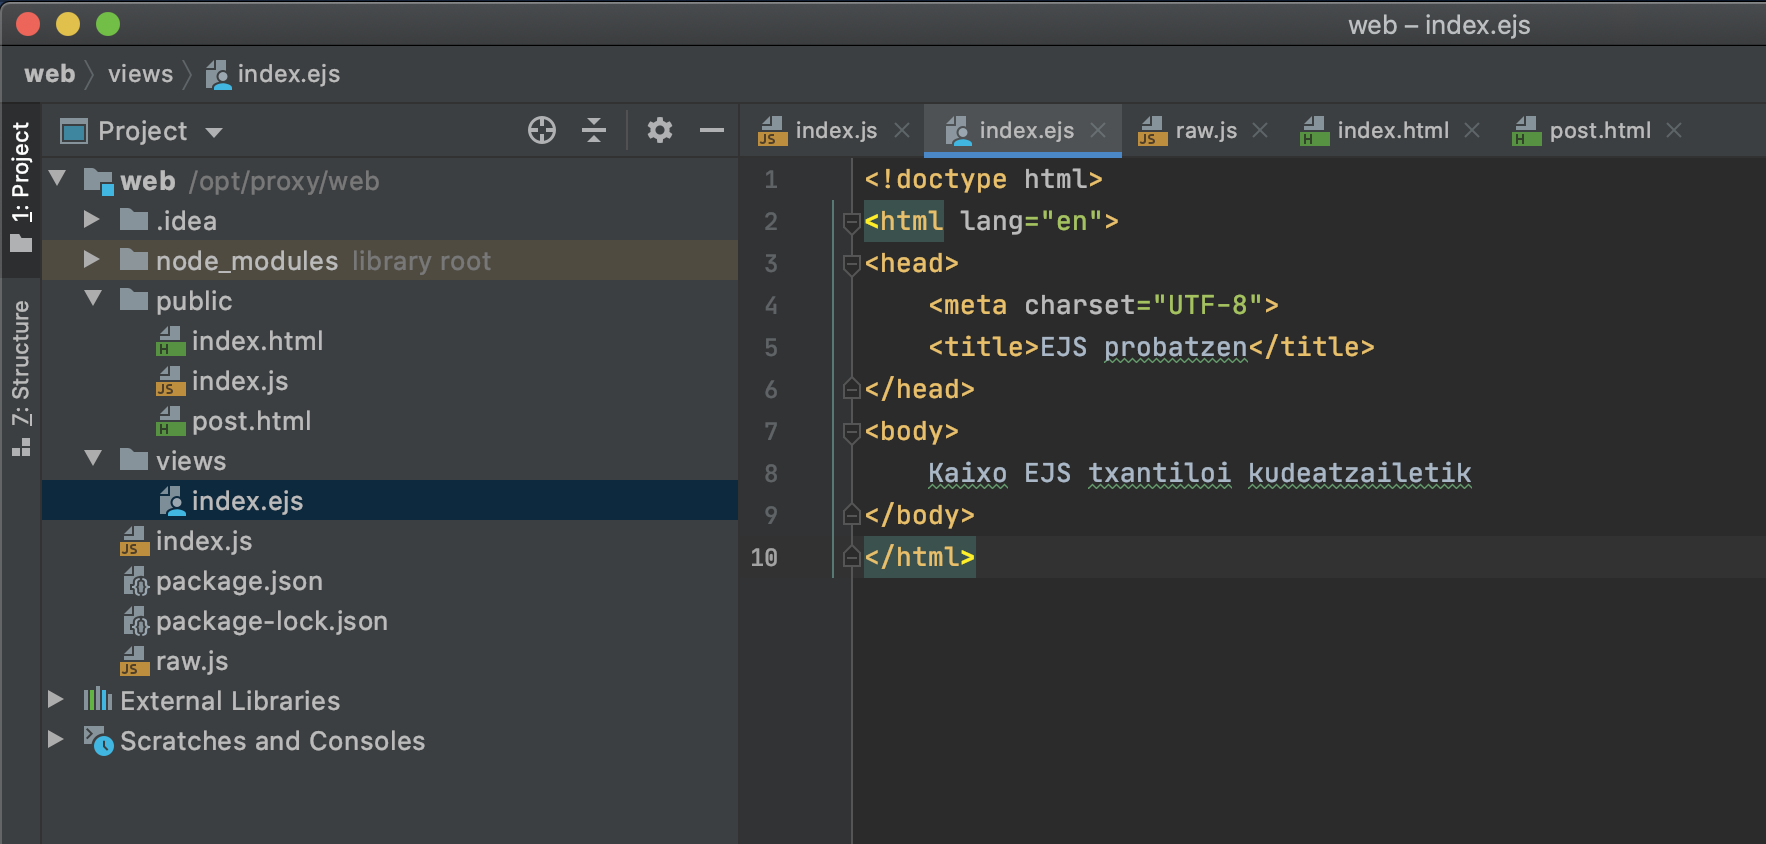
\includegraphics[trim=0cm 0cm 0cm 0cm, clip=true, width=1.0\textwidth]{img/ejs.png}};
\end{tikzpicture}
\caption{EJS txantiloiak probatzeko, \hl{views/} izeneko karpeta bat sortu dugu eta bertan \hl{index.ejs} fitxategia sartu.}
\label{fig:ejs}
\end{figure}

Orain arte ikusi dugunaren arabera, ez dugu inolako aldaketarik somatzen EJS txantiloi baten eta HTML orri estatiko baten aldean (public/ karpetan ditugun orrien artean). Ezberdintasun nagusia da txantiloiek parametroak onartzen dituztela. Adibidez, \hl{app.get(\textquotesingle{}/\textquotesingle{})} kudeatzailetik parametro bat pasatu nahi badiogu txantiloiari, honakoa idatziko dugu \hl{index.ejs} fitxategiaren \textit{title} atalean, izenburua parametro gisa jasotzeko:

\begin{lstlisting}[language=HTML]
<title><%=izenburua %></title>    
\end{lstlisting}

Alegia, EJS aldagai bat \hl{<\% \%>} ikurren artean sartuko dugu. Eta aldagai hori txantiloian bistaratu nahi badugu, \hl{<\%=aldagaia\%> } idatziko dugu.

Bukatzeko, app.get(\textquotesingle{}/\textquotesingle{}) kudeatzailea honela geratuko da:

\begin{lstlisting}[language=JavaScript]
app.get("/", function(req, res) {
    res.render('index', {
        'izenburua': 'Kaixo EJS txantiloi kudeatzailetik'    
    }) 
});
\end{lstlisting}

Txantiloia ondo dabilela probatu baino lehen, \hl{public/} karpetatik \hl{index.html} ezabatu egingo dugu. Ez badugu egiten, \textit{express}-ek hor aurkituko du \textit{index} izeneko orri bat eta hori hobetsiko du txantiloiaren aurrean. 

Dena ondo badoa, \hl{http://localhost:3000} webgunea atzitzean, \ref{fig:txantiloia1-ejs}. irudian ikusten dugun emaitza lortu beharko genuke.

\begin{figure}[ht]
	\centering
\begin{tikzpicture}[framed]
\node[anchor=south west,inner sep=0] (image) at (0,0)
   {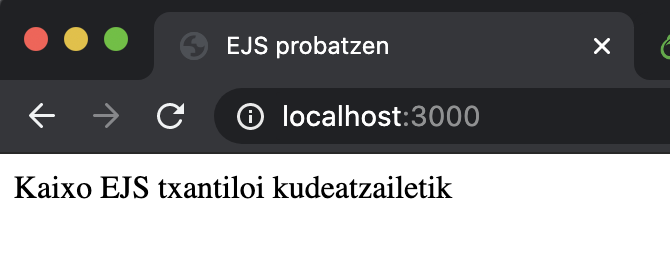
\includegraphics[trim=0cm 0cm 0cm 0cm, clip=true, width=.75\textwidth]{img/txantiloia-ejs.png}};
\end{tikzpicture}
\caption{EJS txantiloiek parametroak onartzen dituzte. Izenburuan ikus dezakegu orri honi pasatu diogun parametroa.}
\label{fig:txantiloia1-ejs}
\end{figure}

\subsection{Txantiloiak betetzen}

Demagun hiru bezeroren datuak ditugula:

\begin{lstlisting}[language=JavaScript]
let bezeroak = [
    {
        id: 1,
        izena: 'Ane',
        abizena: 'Uriarte',
        email: 'ane@ni.eus'
    },
    {
        id: 2,
        izena: 'Jon',
        abizena: 'Juanenea',
        email: 'jon@ni.eus'
    },
    {
        id: 3,
        izena: 'Oihane',
        abizena: 'Lete',
        email: 'oihane@ni.eus'
    },
]
\end{lstlisting}

Orain, datu horiek web orrian bistaratu nahi baditugu, parametro gisa pasa behar dizkiogu \hl{index.ejs} txantiloiari:

\begin{lstlisting}[language=JavaScript]
app.get("/", function(req, res) {
    res.render('index', {
        'izenburua': 'EJS probatzen',
        'bezeroak': bezeroak
    })
});
\end{lstlisting}

Eta index.ejs txantiloian datuak zeharkatu, \textit{forEach}\index{forEach} egitura erabiliz:

\begin{lstlisting}[language=HTML]
<!doctype html>
<html lang="en">
<head>
    <meta charset="UTF-8">
    <title><%=izenburua%></title>
</head>
<body>
    Kaixo EJS txantiloi kudeatzailetik
    <ul>
        <% bezeroak.forEach( function(bezeroa) { %>
        <li><%=bezeroa.izena %> <%=bezeroa.abizena%></li>
        <% }) %>
    </ul>
</body>
</html>
\end{lstlisting}

Dena ondo badoa, \hl{http://localhost:3000/} helbidean sartzean, \ref{fig:txantiloia-ejs}. irudiaren emaitza ikusiko dugu.

\begin{figure}[ht]
	\centering
\begin{tikzpicture}[framed]
\node[anchor=south west,inner sep=0] (image) at (0,0)
   {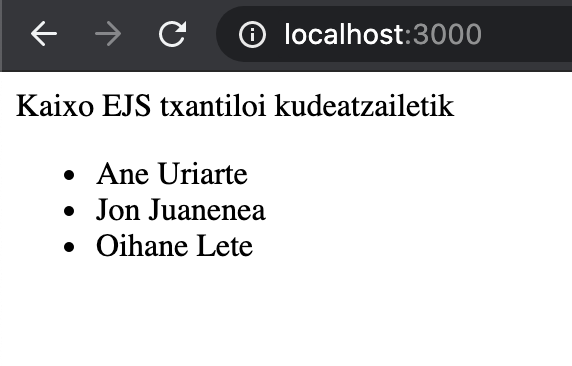
\includegraphics[trim=0cm 0cm 0cm 0cm, clip=true, width=.5\textwidth]{img/ejs-bezeroak.png}};
\end{tikzpicture}
\caption{Bezeroen datuak JSON array batean EJS txantiloiari ondo bidaltzen badizkiogu, honela ikusi beharko litzateke nabigatzailean.}
\label{fig:txantiloia-ejs}
\end{figure}

\section{Ariketa}
Prestatu inprimaki bat \hl{index.ejs} txantiloian, bezero berri baten datuak (izena, abizena eta helbide elektronikoa) zerbitzarira POST bidez bidaltzeko. Zerbitzariak datuak jaso eta pantailan bistaratuko ditu. 

